
\chapter{Implementation of Segmentation, ABCD rules, and Dermoscopic Structures}

\section{Introduction}
This chapter is a discussion of the most popular ABCD (Asymmetry, Border, Colour, and Dermoscopic Features) algorithms including their implementation, and updating the algorithms. They are compared using the PH2 dataset and updated relating to their accuracy. Surprisingly, many of the ABCD rules techniques were originally tested for whether they effectively find melanoma and not individual features. So, this will be the first time some of these techniques have been tested and documented.

%Discuss the ABCD rule techniques and how border is better with a tighter border rather than segmentation from techniques including SegNet
\section{Development of a hybrid segmentation machine learning technique}
Segmentation plays a crucial role in melanoma detection because it separates melanoma from healthy skin. Accurate segmentation is essential for various aspects of melanoma diagnosis, treatment, and classification\cite{Albahli2020}. The accurate recognition of melanoma is a challenging task due to the contrast between lesions and skin, including visual similarities between melanoma and non-melanoma skin lesions\cite{li2018}. The goal of producing segmentation techniques is to simplify and transform the representation of images into a more meaningful form for analysis, which is essential for precise representations of melanoma lesions\cite{Masood2013}. This essentially leads to a more effective diagnosis by identifying key features that indicate malignancy\cite{ali2023}. Furthermore, accurate segmentation supports the development of computer-aided diagnostic (CAD) systems by extracting a relevant area of the skin lesion for analysis and ensuring that the relevant area of the image is classified, improving the accuracy of classification algorithms\cite{bi2019}. Overall segmentation is vital for the accurate and reliable analysis of melanoma, enabling the analysis of melanoma through the extraction of relevant features.

Accurate segmentation also plays a crucial role in analysing ABCD rules\cite{Lee2020}. This is especially vital for the analysis of border features\cite{Pereira2020, Kaya2016} including convexes and indents. The irregularity of borders is a key feature in distinguishing melanoma from benign lesions, and the exact identification of irregular borders from melanoma skin lesions is clinically significant\cite{patil2021}. An accurate border cut-off is also important for the analysis of asymmetry and colour which both classify the colour of the skin lesion. An accurate border is also essential to analysing lesions by preventing skin from accidentally being calculated in the process, ruining the accuracy. It's important to note that many of the ABCD rules algorithms are statistical and highly sensitive to incorrect segmentations.

There are various deep learning approaches\cite{Albahli2020} and deep CNN techniques\cite{yu2017}. These highlight the significance of advanced technologies for accurate segmentation and detection of melanoma. Although these techniques are massively accurate they are trained and tested against datasets (ISIC 2018) containing a mixture of approximate segmentation masks and expert segmentation masks. Shown in figure \ref{seg-expert}, approximate borders are a rough estimation of skin lesion area and expert segmentation masks fit the skin lesion tighter representing border features. The mixture of images results in produced borders from many deep learning techniques having an inaccurate border cut-off border, whilst appearing accurate when tested against datasets. The ISIC 2018 dataset has a mixture of approximate segmentation masks and expert borders, which is not enough to train deep learning algorithms. Furthermore, the images are also shrunk as part of the deep learning process, which in turn loses smaller features that are significant when analysing borders. Various hybrid techniques have been developed using statistical algorithms active contouring-based segmenatation\cite{Riaz2019}, LBPC and others for border adjustment including u-otsu and edge-imfill. Specifically, u-otsu has been previously used to adjust the borders of melanoma to create expert borders\cite{}.

%Show example of borders and expert borders
\begin{figure}[]
    \centering
    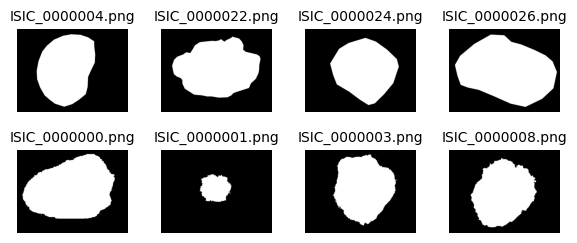
\includegraphics[scale=0.9]{images/segmentation/seg-expert-approx.png}
    \caption{This figure shows examples of different styles of segmentation in the ISIC 2018 dataset with approximate segmentation masks on the top row and expert segmentation masks on the bottom.}\label{seg-expert}
\end{figure}

As shown in figure \ref{seg-expert} expert borders are tighter to the area of the skin lesion and approximate borders are the area of the lesion. Images have either approximate borders or expert borders and no others in the ISIC 2018 dataset, measurements are likely skewered because of the variation in types of borders.

\subsection{Data Organisation}
As mentioned in the previous section the ISIC 2018 dataset contains a mixture of approximate borders and expert borders. The statistical algorithms (U-otsu, LBPC) generate an accurate border cut-off and would have a better accuracy for expert borders, but worse for approximate border. The opposite is true for deep learning algorithms (U-net, SegNet) where they produce approximate borders and should ideally be tested against approximate borders. Considering these problems to better assess the quality of algorithms, the ISIC 2018 dataset is split into expert and approximate masks to better verify the accuracy of techniques.

To automatically split the dataset a simple algorithm is utilised called fractal box-counting which is designed to measure the complexity of a border. 

Out of 2,594 images ... are added to the approximate dataset of ... because they do not have expert borders. However because of the number of images needed to train the algorithms. Considering the deep learning algorithms only produce a rough border they are tested against the approximate borders in the ISIC 2018 dataset. This should allow for a better comparison of the techniques.

After comparing a range of these techniques the two highest performing are combined and tested against the expert

Furthermore, border cut-off is subjective making it challenging to analyse

%Box-counting didn't split the values at all, another method needs to be used

\subsection{Semantic Pixel-Wise Segmentation (SegNet)}
Semantic Pixel-wise segmentation termed SegNet is a deep convolutional encoder-decoder architecture designed for the automatic segmentation of images. It was originally developed in 2015 by Badrinarayanan et al.\cite{} and has shown promising results for various segmentation tasks including those in the medical field. SegNet has been used in a variety of applications in the medical field including lung X-ray abnormality annotations\cite{}, dental imaging\cite{kwak2020}, liver tumor segmentation\cite{Priyadarsini2022}, and many others. It is known for its efficiency in terms of memory and computational time and is known for being more memory efficient than other architectures including U-Net\cite{Mirzazade2021}. Further developments have been made in upgrading SegNet into different versions including Bayesian SegNet\cite{Dhanagopal2022}, VGG-SegNet\cite{}, and ResNet-SegNet\cite{}, with differences in the encoder and decoder layers.

The engine consists of an encoder network with identical 13 convolutional layers. The idea of SegNet is to perform pixel-wise classification by assigning each pixel in an image to a specific class or category. This is achieved through a deep convolutional encoder-decoder architecture, which allows for robust semantic pixel-wise labelling.

Semantic pixel-wise segmentation (SegNet) is a machine learning architecture utilizing a deep, fully convolutional neural network (DCNN). This network requires training from ground truth and pre-segmented images for automatic segmentation. SegNet consists of encoding layers, decoding layers, and a pixel-wise classification layer. The encoder layers consist of 3$\times$3 convolutions (including batch normalization and ReLU), and pre-trained filters for classifying features. After some convolutions, the data is down-sampled using a 2$\times$2 pooling layer. Next, decoding layers consist of up-sampling, followed by 3$\times$3 convolutions. Finally, the pixel-wise classification uses a softmax layer to represent each pixel between 0 and 1 based on the previous layers, generating a segmentation mask.

%Explain training parameters
In evaluating the effectiveness of a trained model, several training parameters are commonly used. These parameters serve as quantitative measures to assess the performance of models. The following parameters are utilised:
\begin{itemize}
    \item Loss: The loss function is a parameter used to measure the inconsistency between the predicted segmentation and the ground truth. Loss is typically minimised as the model is trained through the optimisation algorithm including Adam or stochastic gradient descent (SGD).

    \item Recall: The recall function otherwise known as sensitivity evaluates the ability of the model to correctly identify instances within an image. For example, it is calculated as a true positive to the sum of true positives and false negatives. A high recall value means that the model is effective at capturing the relevant objects in the image.

    \item Accuracy: The accuracy is a fundamental metric that measures the overall correctness of the model's classification. It is calculated by the number of correct predictions to the total number of number of predictions. Accuracy tends to be ineffective in analysing unbalanced datasets.

    \item The precision quantifies the accuracy of the model's positive predictions. It is calculated as the true positive to the sum of true positives and false positives. A high precision indicates that the model has a low risk of producing false positive predictions.

    \item Dice Coefficient: The dice coefficient that is also known as F1 score is a metric that combines precision and recall into a single value. It is calculated as the harmonic mean of precision and recall. This provides a balanced assessment of general model performance in segmenting images.

    \item Jaccard Index: The Jaccard index or Intersection over Union (IoU) measures the similarity between the predicted segmentation and ground truth. It is calculated with the intersection of the predicted and ground truth regions to the union, providing the model's segmentation accuracy.
\end{itemize}

These parameters are a collective evaluation of the SegNet model's performance in image segmentation. These allow researchers to assess the effectiveness of the models and how they might function in real-world scenarios.

\begin{figure}[]
    \centering
    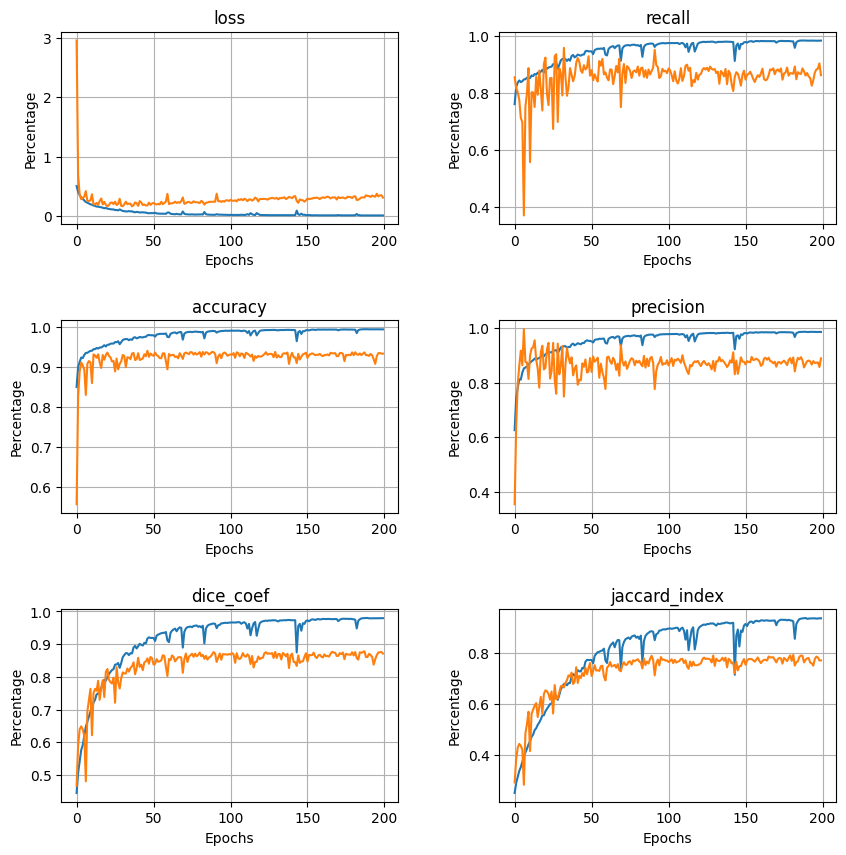
\includegraphics[scale=0.7]{images/segmentation/SegNet-results.png}
    \caption{}\label{SegNet-results}
\end{figure}

%Share results
After training the model using parameters and 100 epochs the trained model has the following metrics, shown in figure \ref{SegNet-results}.

\begin{figure}[]
    \centering
    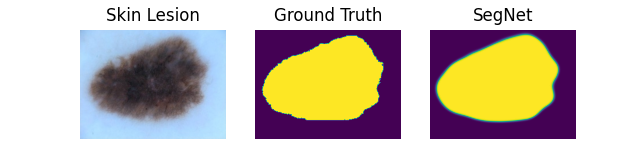
\includegraphics[scale=1.0]{images/segmentation/SegNet-1.png}
    
\includegraphics[scale=1.0]{images/segmentation/SegNet-2.png}
    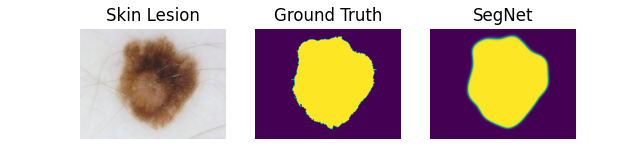
\includegraphics[scale=1.0]{images/segmentation/SegNet-3.png}
    \caption{SegNet model segmentation compared with the skin lesion, ground truth, and segmentation.}\label{SegNet-examples}
\end{figure}

Here are some examples of the SegNet model described in figure \ref{SegNet-examples}. SegNet appears to capture the area of the skin lesion to a high accuracy, but when compared with the expert borders in the images it fails to capture these features.

Results in figure \ref{SegNet} are generated from the architecture using the ISIC 2018 dataset split into 80\% training and 20\% validation images. The accuracy of locating the lesions is 85\%. However, it represents the border cut-off between skin and skin lesion accurate to the dataset but inadequate for using the ABCD rules. Finding the border cut-off is vital for measuring ABCD rules\cite{Pereira2020}.

\subsection{Unet}
%Consider removing because there is very little time
U-net or U-shaped neural network is a deep neural network (DNN) architecture that gained significant attention, particularly in medical image segmentation. 

that was developed for the automatic image segmentation of images. It is an encoder-decoder architecture designed for semantic segmentation tasks, it is especially useful for medical image analysis\cite{zhou2020}.  

\subsection{Otsu Threshold}
Otsu threshold is a versatile automatic image thresholding technique meant to separate each pixel between two classes of foreground or background. One of the benefits of this method is that it does not require any training data. The equation \ref{otsu} (within-class variance) describes splitting weights of $w_0(t),w_1(t)$, which are the probabilities divided by the threshold $t$, between 0 and 255. Furthermore, $\sigma_1^2$ and $\sigma_0^2$ are variances of these two classes. The class probability $w$ is computed from the histogram in figure\ref{otsu2}, which is an intensity histogram describing the colour distribution in an image. Measuring the values above and below the generated thresholds splits the image into two classes.

\begin{equation}
\sigma_w^2(t) = w_0(t)\sigma_1^2(t) + w_1(t)\sigma_2^2(t)
\end{equation}\label{otsu}

The histogram was split into two segments with the threshold $t$ of 138 and the corresponding pixel locations to the histogram segment the skin lesion into two classes. Image morphology closing was applied to fill gaps that the threshold missed. On other occasions, the segmentation missed the skin lesion because of a similar colour between the skin and the skin lesion. It might be beneficial to combine Otsu with SegNet to improve its accuracy while producing a border cut-off. Figure\ref{otsu2} describes the difference between otsu and SegNet.

\begin{figure}
\centering
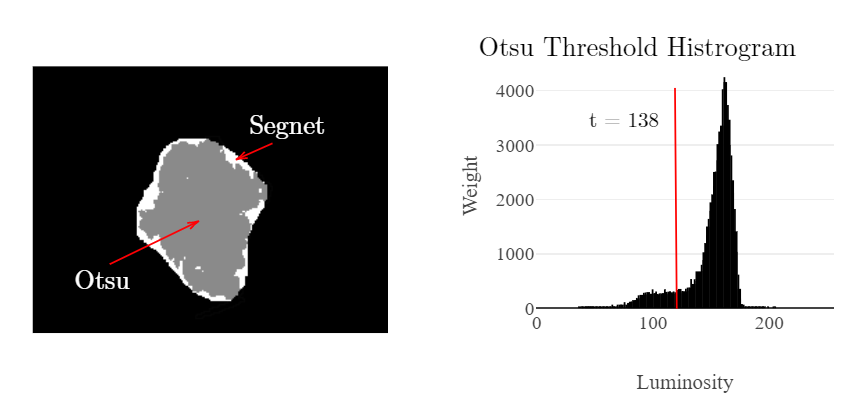
\includegraphics[scale=0.7]{images/otsu3.png}
\caption{Otsu thresholding alongside ground-truth mask, where grey Otsu and white is SegNet. The bar chart shows the histogram with an otsu threshold of 138.}\label{otsu2}
\end{figure}

\subsection{Local Binary Pattern clustering (LBPC) Segmentation}
Local Binary Patterns (LBP) is a texture descriptor commonly used for augmenting the image improving classification accuracy\cite{Pereira2020, Kaya2016}. First, equation\ref{eq1} calculates each pixel, where $p$ (equal to 8) is the number of neighbouring pixels compared to the centre of $c$, and the radius of $r$ from the centre. Next, shown in equation\ref{eq2} each value is subtracted counter-clockwise with the centre value and compared to function $S$ where each $gp - gc$, if more than or equal to 0, is equal to 1, and less than 0 is equal to 0. Next, add corresponding values equal to 1 of $gp$ together, changing the centre value, ignoring values of 0. Next, applying a Gaussian kernel of 13-pixel iterations and a standard deviation of 3 removes smaller features that interfere with the segmentation. Finally, applying k-means with a value of 2 subtracts the greyscale and segments the skin lesion from the skin.

\begin{equation} \label{eq1}
LBP(gp_x, gp_y) = \mathlarger{\sum}_{p=0}^{P-1}s\big(gp - gc)2^p
\end{equation}

\begin{equation} \label{eq2}
s\big(x) = 
\begin{cases}
1,\:\:x\geq\:0; \\
0,\:$otherwise$.
\end{cases}
\end{equation}

Figure \ref{fractal1} demonstrates the segmentation of two skin lesions, one with an irregular border and another with a regular border. LBPC is applied to both skin lesions, followed by Gaussian blurring and morphology closing to remove dots. The result is an improved border cut-off compared to the ground truth in the Ph$^2$ dataset with more corners and ledges. This technique will improve accuracy for measuring border irregularity\cite{Pereira2020}.

\begin{figure}
\centering
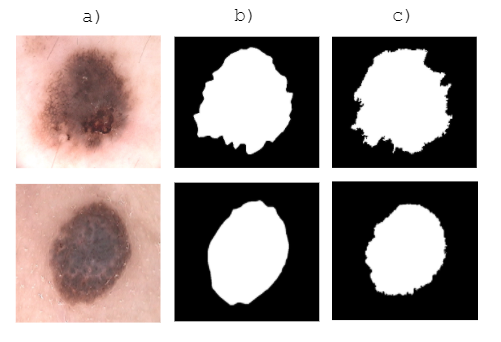
\includegraphics[scale=1.2]{images/borders.PNG}
\caption{Local Binary Pattern Clustering (LBPC) showing the a) original image, b) ground-truth, and c) LBPC. LBPC successfully exaggerates the border cut-off on the skin lesions with regular and irregular borders} 
\end{figure}\label{fractal1}

Validating LBPC is not expected because the goal is to exaggerate the border to improve the classification process of ABCD rules, which it does successfully\cite{Pereira2020, Kaya2016}. For example, the segmentation might not match dataset segmentations but is still essential to classifying ABCD rules. Furthermore, many datasets lack expert border segmentation, an accurate border cut-off between the skin and skin lesions, so comparisons are not always possible.

\subsection{Results}
Overall the accuracy of the techniques demonstrates that SegNet is the most reliable technique. However, comparing the techniques in \ref{} we can demonstrate that it produces a smudge effect and fails to capture the border cut-off from the skin lesion, but it is successful at finding the location of the skin lesion.

Both statistical models of LBPC and Otsu threshold generated an accurate border cut-off between the skin and the skin lesion As previously mentioned, measuring the border cut-off and exaggerating irregular borders are helpful when calculating the ABCD rules. 

It might be beneficial to combine SegNet and LBPC using SegNet to find the skin lesions' location, followed by adjusting the border cut-off using LBPC. A similar technique using the Otsu threshold and Segnet is described by Riaz et al.\cite{Riaz2019}.

\begin{figure}
    \centering
    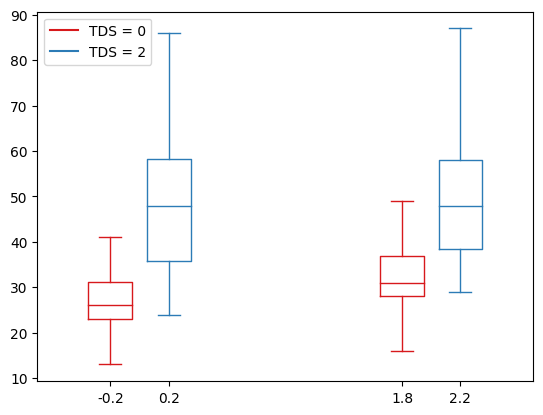
\includegraphics[scale=1.2]{images/asymmetry/asy-changes.png}
    \caption{} 
\end{figure}\label{asy-changes}

Figure\ref{asy-changes} demonstrates the difference between the updated asymmetry algorithm using super pixels compared with the original


the asymmetry algorithm using super pixels decreases the median and range, compared with the original method where the pixels are closer together

%Tables showing the accuracy of all three of the techniques essentially showing that segnet is obviously better.

\subsubsection{Border Cut-off}
%Show that regardless of segnet being better that the other techniques still have a better border cut-off improving border irregulrity detection
This section includes a simple border analysis technique called fractal box counting to assess the benefits of using different segmentation algorithms with accurate border cut-offs.

To prove the usefulness of segmentation techniques with an accurate border cut-off a technique developed by Ali\cite{Ali2020b} is implemented that utilises machine learning with extracted data including Zernike moments, fractal box-counting, and convexity measurements. Fractal box-counting is used to measure the irregularity of the border.

The fractal box-counting technique is a commonly employed technique for analysing fractal properties. It involves dividing a fractal object or pattern into a grid of equally sized boxes and counting the number of boxes that contain a portion of the fractals. The process is repeated with different box sizes until the boxes until the relationship between the box sizes and the number of boxes is analysed determining the fractal dimension\cite{Hamburger1996}. Essentially a more complicated border with corners and convexes will have more boxes and therefore a higher fractal score, than for example a border with smooth corners and edges which has a lower score. This should provide some evidence of the usefulness of an accurate border.

\subsection{Issues}
%Show that LBPC sometimes fails at finding the skin lesion
The segmentation algorithms encountered some issues, whilst the best of the techniques was SegNet with an 85\% accuracy when relating to the ISIC 2019 dataset. However, as previously mentioned the segmentation masks have poor border cut-off stunting features that are useful for finding border irregularities. 

In contrast LBPC and U-Otsu algorithms effectively identify the border cut-off of the skin lesion, which isn't properly represented in the ISIC 2019 dataset. But, it sometimes fails to find the skin lesion or not detect anything. 

Both techniques appear to have downfalls making them less effective for use for analysing ABCD rules. It would be beneficial to find the approximate area of the skin lesion using SegNet and followed by LBPC to find the border cut-off.

\section{Joint Neural network and statistical model approach}
%Combine techniques together to get the area of the border


Combining both SegNet and LBPC improves the accuracy. 


















\section{ABCD Rules Data Extraction Techniques}
The automatic detection of ABCD rules for the detection of ABCD rules has warranted extensive research and development\cite{Ali2020}. The ABCD rules stand for Asymmetry, Border irregularity, Colour variegation, and Diameter greater than 6mm, and have been fundamental framework for the clinical diagnosis of melanoma. Sometimes Diameter is changed for Dermoscopic structures because measruing the size of the lesion is not always possible when capturing an image. Furthermore, demroscopic structures provides further insight into diagnosing melanoma\cite{}. Another useful change made to the ABCD rules is E for evolution, showing that it changes overtime, datasets however do not support this. Although the diagnostic procedures ABCD rules is frequently used in the medical environment it has limitations in detection of small melanomas and those with resular shape and homoheneous colour\cite{Argenziano2006}. As a result, automatic classification algorithms for ABCD rules has become more prevelant\cite{Kasmi2016}.

Some of the benefits of implementing a CAD system for the automatic detection of ABCD rules is the the classification of exisiting diagnostic procedure in which clinicians are already aware of how it fundementally works. Another benefit is the automatic labelling of data, where it would take considerable time to input this diagnostic data into a server for further analysis, where the automatic system could generate results and the clinician only needs to check whether these results are correct. Other benefits include improving objectivity of results, where normally ABCD rules is considered subjective, meaning it can be utilised in a variety of ways. This ultimietly makes comparisons very difficult between lesions, but automatic detection can improve the objectivity, making hospital wide comparisons easier. Check out the previous chapter discussing the PH2 dataset and the data subjectivity on page\pageref*{ph2-image-assessment}.

\subsection{Asymmetry Techniques}
Asymmetry analysis is a fundamental component in the early detection of melanoma because it often exhibits asymmetric shapes\cite{Ali2020a}. Meaning that the shape, colour and, texture match asymmetrically more often in benign lesions. For example, as melanoma grows the central area begins to waste away leaving a hollow area covered by thin skin, showing dermoscopic features. As it grows the edges become more irregular producing an uneven shape often relating to irregular borders and asymmetrical shapes. Diagnostic procedures have been developed to detect these unique characteristics.

\begin{figure}
    \centering
    %\includegraphics[scale=1.2]{images/asymmetry/.png}
    \caption{} 
\end{figure}\label{asy-examples}


\section{A Novel Asymmetry detection technique using Bi-Fold, 3D Euclidean distance, and Superpixels}
This section describes a novel machine-learning technique for the automatic detection of melanoma

\subsection{Image Transformation}
Transforming the skin lesion image is important to prevent scale variance in the algorithms. For example some of the images have a smaller skin lesion in upper corners and others take up the entire image size. For adequate comparisons the images must be transformed to match sizes. THis ensures the images are being compared fairly.

To transform the image it is converted to gray scale and a threshold is applied finding all non-zero pixels. This is followed by a bounding rectangle around the area being assigned. After this the assigned area from the original image is cropped.

\begin{figure}
    \centering
    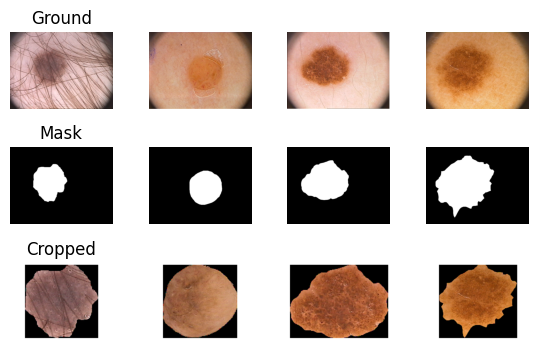
\includegraphics[scale=1.2]{images/asymmetry/asy-cropped.png}
    \caption{This figure shows some images from the PH2 dataset after being masked, cropped, and rotated using bi-fold.} 
\end{figure}\label{asy-cropped}

%Diagram showing the image before and after transformation
The first line in figure \ref{asy-cropped} shows the skin lesion image, the second shows the segmentation mask, and the third shows the images after being cropped and rotated using bi-fold.

\subsection{Bi-fold}
Bi-fold is a diagnostic procedure designed to support the recognition of melanoma by drawing a line down the middle of the skin lesion and comparing the two halves to confirm whether the sides match (considering the difference in shape, colour, and texture). Using this horizontally and vertically calculates whether the skin lesion is possibly malignant with a score between 0 and 2. Calculating with Total Dermoscopy Score (TDS) alongside the other ABCD rules including asymmetry, border, colour, and diameter calculates the likelihood of malignancy. Dermatologists frequently use bi-fold due to its simplicity, but it can be subjective to the original observer and time-consuming when managing large numbers of skin lesions. Therefore, automating techniques is beneficial to clinicians and can improve the objectivity of results.

To initiate the classification of skin lesions a technique called bi-fold is applied involving folding the skin lesion in half vertically and horizontally and a comparison of their respective dimensions. While the original technique was designed only to assess the lesions' shape, it's been utilized to account for colour and texture as well. The centre and orientation are determined by calculating its moments, where the centre is (m10 / m00, m01 / m00) and phi is 0.5tan (2m11)/ (m20 -m02).

%Add diagram demonstrating bi-fold of a skin lesion
\begin{figure}
    \centering
    %Make better images showing both vertical and horizontal rotation after analysis
    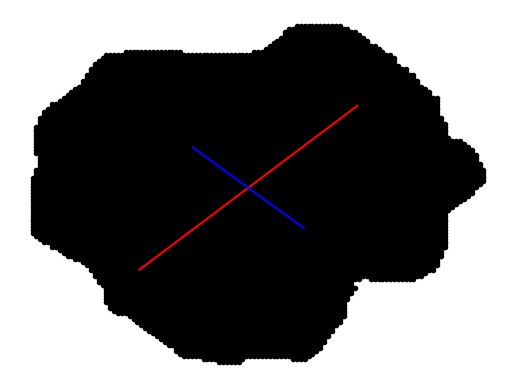
\includegraphics[scale=0.5]{images/asymmetry/bi-fold1.png}
    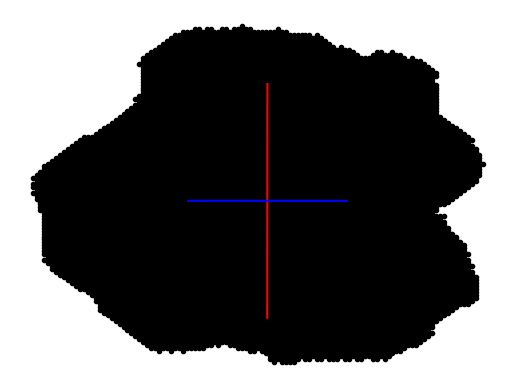
\includegraphics[scale=0.5]{images/asymmetry/bi-fold1-rotated.png}
    \caption{This diagram shows image IMD003 from the PH2 dataset after calculating Bi-fold, followed by rotating the image to match the rotation defined using moments of inertia.} 
\end{figure}\label{asy-bifold}

\subsection{Shape analysis}
Analysing the shape of the skin lesion 

\subsection{3D Euclidean Distance}
Next, the lesion is partitioned into a 20 by 20 grid centred on the mentioned centre point, and the average of each region is computed. This is followed by finding the matching region on the perpendicular area from the centre of the skin lesion and comparing the colour distance between the two. Distance is measured using the LAB colour space and a 2D Euclidean distance of A and B, removing L (luminosity) to eliminate light variation. Once compared, all compared regions are obtained, and they are plotted onto a graph. If over half of the values are above a threshold of 6, then the lesion is asymmetrical.

% Scrutinize the threshold method and show the graph that the data can't be split with only the threshold 
The diagram shown below in figure\ref{symmetrical} is a compilation of all the images within the PH\^2 dataset showing the threshold range after applying bi-fold, euclidean distance of colour, but before applying the threshold. As can be seen, a threshold of 6 covers all of the symmetrical values, but still roughly covers half of the asymmetrical values. This demonstrates that the technique produces many false positives when regarding asymmetrical values.
Essentially, the symmetrical skin lesion has a smaller area and the asymmetrical lesion has a larger area, but both remain in the same zone and therefore splitting the data only using a threshold holds poor results. Furthermore, there are a lot of fliers and the threshold does not adjust according to these values. See the graph below:

\begin{figure} 
    \centering
    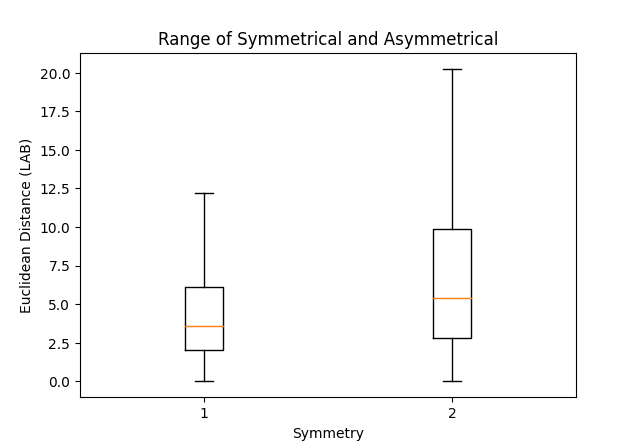
\includegraphics[scale=0.6]{images/symmetrical.png}
\caption{This diagram is a summary of the PH2 dataset after using bi-fold, a Euclidean distance of colour. The value on the right would be a threshold.}
\end{figure}\label{symmetrical}
    
To improve the accuracy of the algorithm some changes need to be made based on the previous statements. First will be superpixels and next is k-means.

\subsection{Superpixels using Simple Linear Iterative Clustering (SLIC)}
% Demonstrating the changes including superpixels and graphs, etc
Superpixel is an algorithm for grouping pixels into a grid format, but with flexible borders that can adjust to regions with similar features. Unlike the original technique averaging specific squares in a grid\cite{Kasmi2016}, they are segmented related to colour, texture, and other properties. The reason for using this technique is to increase boundary adherence and to group features that might otherwise be split into separate groups. This overall improves the accuracy of the algorithm.

This technique uses a simple linear iterative clustering (SLIC) algorithm and was first introduced by Achanta et al.\cite{Achanta2012}. The technique combines both k-means and graph-based segmentation. Firstly you define the desired number of superpixels as $k$ and the approximate size of each superpixel as $S$, which is usually $S = /square(N/k)$ and $N$ is the number of pixels in the image. Secondly, for the centre of each cluster, a search space is assigned to the cluster. For each group, you measure the spatial distance which is the Euclidean distance between each pixel and the cluster center. Each pixel is assigned to the cluster with the nearest centroid. The cluster centres are then recalculated by taking the mean colour and position of the pixels assigned to each cluster. Followed by new pixels being assigned to the centroid relating to Euclidean distance. This process is repeated depending on the number of iterations as $i$ are assigned. From this point, each pixel is assigned to a cluster.

The image in ... demonstrates the usual average and the new averages based on superpixels and the changes in values. Areas that are lighter in colour appear to have a lower value and darker appear darker.

Using the thresholding method for classification we can already see the accuracy has been improved with a threshold of ...

\section{Experimental Results}
The goal of this experiment is to improve the accuracy of the asymmetry bi-fold technique described by Ihab S. Zaqout et al.\cite{Zaqout2016}. Initially, the skin lesion is split into a 10 by 10 grid and converted into the LAB colourspace. Next, a line is drawn through the middle horizontally and vertically. Measuring the Euclidean distance from the centroid, locating the closest opposite patch of colour finds the parallel square. Subtracting the squares generates a score for each value, the closer to 0, the more similar the colour. These are then removed from the list to prevent them from being selected a second time. If half the results are over a specific threshold, it is considered asymmetrical in colour, otherwise considered symmetrical. The aim is to make a 10 by 10 grid, but instead of averaging squares, superpixels reduce data redundancy in the grid, allowing for a less complex algorithm and improving accuracy. The clustering method k-means partitions each pixel to its nearest most similar centroid relating to colour. Next, it generates a superpixel that represents the average colour of that area. The diagram\ref{SP} demonstrates different borders when changing the $C$ for compactness, where 100 generates a square grid similar to the original technique. The border becomes more flexible as the compactness value decreases.

\begin{figure} 
\centering
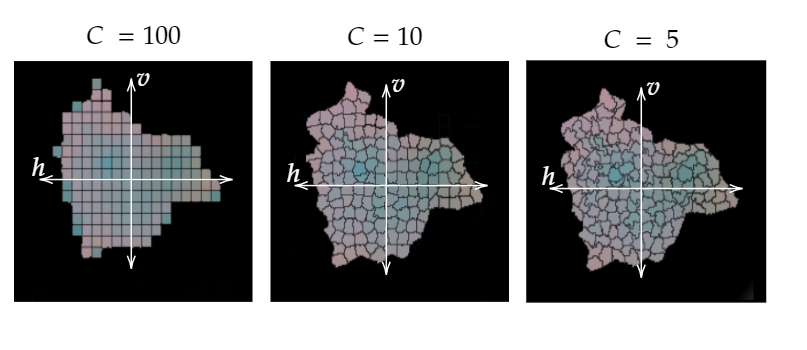
\includegraphics[scale=0.6]{images/superpixels.png}
\caption{This diagram shows the skin lesion split relating to superpixels instead of averaging squares.}
\end{figure}\label{SP}

Each parallel square on the vertical and horizontal axes measures similarity using a three-dimensional Euclidean distance in the LAB colour space. For example, the perceivable difference of colour to the human eye is a three-dimensional Euclidean distance of 6\cite{Myridis2014a}. Using similar logic, a value of 20 is the threshold, where any value over that amount is considered asymmetrical in colour. Next, each square is compared with its closest parallel square (relating to the line through the centre defined by the bi-fold) and removed from an array after being compared. The next improvement is to generate a unique threshold for the significance of each square. For example, using superpixels with the compactness of 10 has an accuracy of 61\% with the PH$^2$ dataset compared to the original 59.5\%. This approach demonstrates that a flexible border that considers features is more effective than averaging squares.

\begin{figure}
\centering
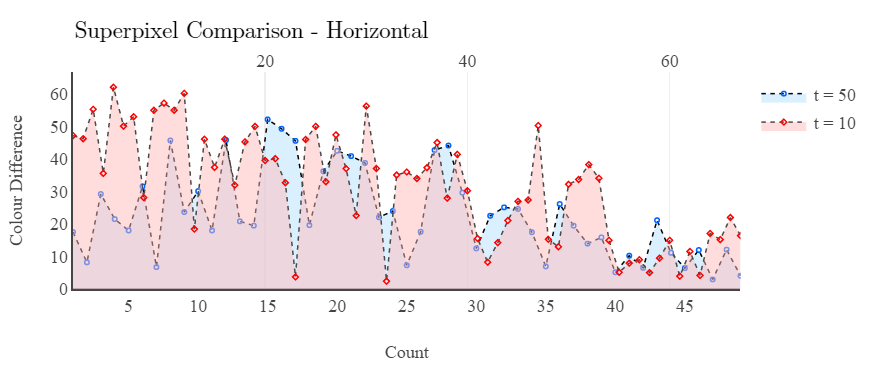
\includegraphics[scale=0.7]{images/superpixel2.png}
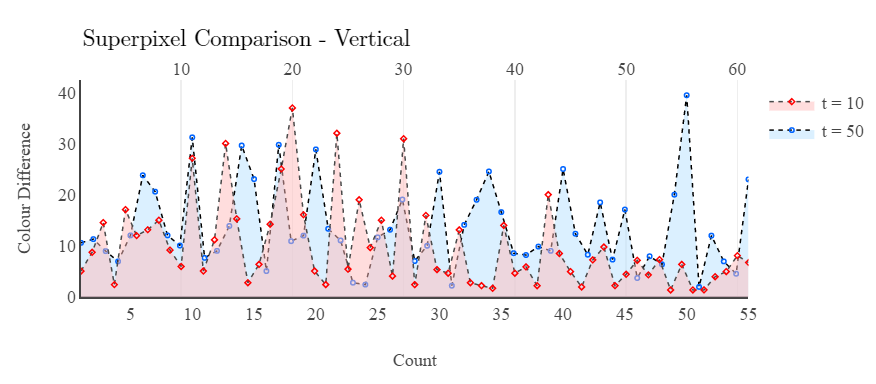
\includegraphics[scale=0.7]{images/superpixel1.png}
\caption{This diagram shows the difference between averaging squares and using superpixels, with the threshold of 10 implying curves and 50 being squares. The horizontal colour difference is improved, making it more likely to be seen asymmetrical. The vertical comparison is roughly the same, except for removing a false positive of 40.}
\end{figure}\label{asy3}

There is a correlation in colour differences between the inner and outer edges because melanoma typically expands outwards, creating an abnormal border. This information specifies that the statistical model accuracy could be improved by increasing the threshold for the outer edges and decreasing it for the inner.

\section{Border Detection Using Zernike Moments, 
Fractal Box-Counting, and Convexity}


\section{A Novel Colour Analysis Approach using Colour Ranges, and SVM}


\section{Dermoscopic structures}

\section{Results}


\section{Conclusion}

% Describe the asymmetry technique and the changes that have been made to it.

%The proposed method has many similarities to Kasmi and Mokrani\cite{Kasmi2016} colour comparison technique, except it is updated to improve accuracy using superpixels, and a Support Vector Machine (SVM).

%The original method uses moments of inertia

%without any flexibility splits areas of interest in half, making comparisons less adequate. Using superpixels allows for a softer border which improves colour separation and accuracy.

%Superpixels are k-means colour extraction techniques designed to separate areas of an image into their associated areas of colour by applying a soft border around the edge.